%----------------------------------------------------------------------------------------
%	PACKAGES AND THEMES
%----------------------------------------------------------------------------------------

\documentclass{beamer}

\mode<presentation> {

%\usetheme{default}
%\usetheme{AnnArbor}
%\usetheme{Antibes}
%\usetheme{Bergen}
%\usetheme{Berkeley}
%\usetheme{Berlin}
%\usetheme{Boadilla}
%\usetheme{CambridgeUS}
%\usetheme{Copenhagen}
%\usetheme{Darmstadt}
\usetheme{Dresden}
%\usetheme{Frankfurt}
%\usetheme{Goettingen}
%\usetheme{Hannover}
%\usetheme{Ilmenau}
%\usetheme{JuanLesPins}
%\usetheme{Luebeck}
\usetheme{Madrid}
%\usetheme{Malmoe}
%\usetheme{Marburg}
%\usetheme{Montpellier}
%\usetheme{PaloAlto}
%\usetheme{Pittsburgh}
%\usetheme{Rochester}
%\usetheme{Singapore}
%\usetheme{Szeged}
%\usetheme{Warsaw}

% As well as themes, the Beamer class has a number of color themes
% for any slide theme. Uncomment each of these in turn to see how it
% changes the colors of your current slide theme.

%\usecolortheme{albatross}
%\usecolortheme{beaver}
%\usecolortheme{beetle}
%\usecolortheme{crane}
%\usecolortheme{dolphin}
%\usecolortheme{dove}
%\usecolortheme{fly}
%\usecolortheme{lily}
%\usecolortheme{orchid}
%\usecolortheme{rose}
%\usecolortheme{seagull}
%\usecolortheme{seahorse}
%\usecolortheme{whale}
%\usecolortheme{wolverine}

%\setbeamertemplate{footline} % To remove the footer line in all slides uncomment this line
%\setbeamertemplate{footline}[page number] % To replace the footer line in all slides with a simple slide count uncomment this line

%\setbeamertemplate{navigation symbols}{} % To remove the navigation symbols from the bottom of all slides uncomment this line
}

\usepackage{graphicx} % Allows including images
\usepackage{booktabs} % Allows the use of \toprule, \midrule and \bottomrule in tables
\usepackage{amsmath}
\graphicspath{{figs/}}
\usepackage{multirow}

\usepackage{tikz}

\let\Tiny\tiny
\usepackage{graphicx}
\usepackage{xmpmulti}
\usepackage{multimedia}
%\usepackage{media9}

%----------------------------------------------------------------------------------------
%	TITLE PAGE
%----------------------------------------------------------------------------------------

\title[DBMS]{Customer Analytics} % The short title appears at the bottom of every slide, the full title is only on the title page

\author{Saumya Bhatnagar} % Your name
%\institute[Data Engineering] % Your institution as it will appear on the bottom of every slide, may be shorthand to save space
%{
%University of California \\ % Your institution for the title page
%\medskip
%\textit{john@smith.com} % Your email address
%}
\date{\today} % Date, can be changed to a custom date

\begin{document}

\begin{frame}
\titlepage % Print the title page as the first slide
\end{frame}


%----------------------------------------------------------------------------------------
%	PRESENTATION SLIDES
%----------------------------------------------------------------------------------------

%------------------------------------------------


\section{Customer Analysis}
\subsection{Churn and LTV}

\begin{frame}\frametitle{Churn or Retention Analysis}
Customer Retention Rate: The percentage of customers who repurchase in a given time period compared to an equal and preceding time period\\
Churn Rate: The inverse of Customer Retention Rate, or the percent of users who did not repurchase or whom you lost\\

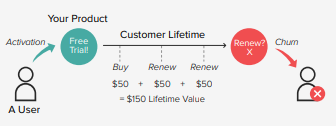
\includegraphics[scale=0.5]{churn}\\
\textbf{proactive churns}: losing customers due to cancellations\\ \textbf{passive churn}: failures to renew\\
\end{frame}


\begin{frame}\frametitle{Cohort Analysis and Life Time Value (LTV)}
\textbf{LTV}: The expected amount of profit/revenue from a user\\
CLV = NPV (net present value) of the sum of all future revenues from a customer, minus all costs associated with that customer\\
\textbf{Why LTV}:
- Tracking your LTV to Customer Acquisition Cost (CAC) ratio: Companies typically use the 3:1 CAC ratio or Cost Per Acquisition (CPA)\\
- Evaluating your most valuable marketing channels\\
- Focus on retaining your most valuable customers\\
\textbf{Historic CLV}: sum of the gross profit from all historic purchases for an individual customer


\end{frame}

\begingroup
\small

\begin{frame}

\begin{table}
\begin{tabular}{llll}
%\hline
\multicolumn{2}{c}{Avg Order Value, AOV = $\frac{Revenue}{Orders}$};
& \multicolumn{2}{c}{Avg Purchase Rate = $\frac{Orders}{NumCustomers}$} 
\\ \hline
\multicolumn{3}{c}{Avg Customer Value = $\frac{Avg Purchase Val}{Avg Purchase Rate}$}
& \multirow{2}{*}{gives LTV}
\\ %\hline
\multicolumn{3}{c}{Avg Customer Lifespan = $\frac{Sum Customer Lifespans}{Num Customers}$}
& \\ \hline
\multirow{5}{*}{LTV = }
& \multicolumn{3}{l}{Avg Customer Value X Avg Customer Lifespan}
\\ 
& \multicolumn{3}{l}{ARPU X $\sum_{n=0}^{N}(1-CR)^t$ .... [N=num months to examine]}
\\
& \multicolumn{3}{l}{ARPU/$CR_n$ ...[ARPU=Avg rev per User, for n months]}
\\
& \multicolumn{3}{l}{ARPU/$CR_n$ x DR ......... [for variable churn \& n months]}
\\
& \multicolumn{3}{l}{ASP/CR + m(1-CR)/$CR^2$ ... [for account expansion]}
\\ \hline
\multirow{3}{*}{CLV = }
& \multicolumn{3}{l}{AGM x $\sum_{0}^{numTransactions} Transaction$ [AGM=Avg Gross Margin]}
\\
& \multicolumn{3}{l}{(($T_{avg}xAOV$)AGM)ALT =GML(gross margin per user lifespan)}
\\
& \multicolumn{3}{l}{GML(R/(1+D-R)); [account expansion]}
\\
\hline
\end{tabular}
\end{table}


CR=Churn rate; ASP=Avg Selling Price; m=$\uparrow$ARPU/user/month;\\
T\_avg = avg monthly transactions; ALT=avg User Lifespan (in months)\\
D=monthly discount rate; R=monthly retention rate; 
DR=Discount Rate to adjusts for mix churn (Annual Renewals, Constant, Declining and Cliff patterns)

\end{frame}

\endgroup

\begin{frame}
Steps to LTV:
\begin{itemize}
\item Normalizing to Acquisition Date: Bin users into buckets like Day 0, Day 1, Day 2 or Week 0, Week 1, Week 2, and so on.
\item Normalized to a Closed Time Limit: Broader questions  “What is my total CLTV,” should be replaced with “What is our 3-year or 5-year LTV?” \& should be based on:
\begin{enumerate}
\item Average Customer Lifespan
\item Customer Retention Rate
\item Churn Rate: The inverse of Customer Retention Rate.
\item Time to General Profitability Against Acquisition Costs: If your business is a “Loss Leader” Model this time may be a longer length than businesses with lower acquisition costs and lower profitability.
\item Rate of Discount		
\end{enumerate}

\end{itemize}
\end{frame}

\begin{frame}\frametitle{Types of churn and LTV}
\begin{itemize}
\item Annual Renewals: larger churn at each contract renewal.
\item Cliff churn: majority of the churn within the first month, and then a small constant churn thereafter.
\item Constant: steady, constant churn rate (shown as 3.5\%).
\item Declining: churn rate starts at zero, increases each month.
\end{itemize}
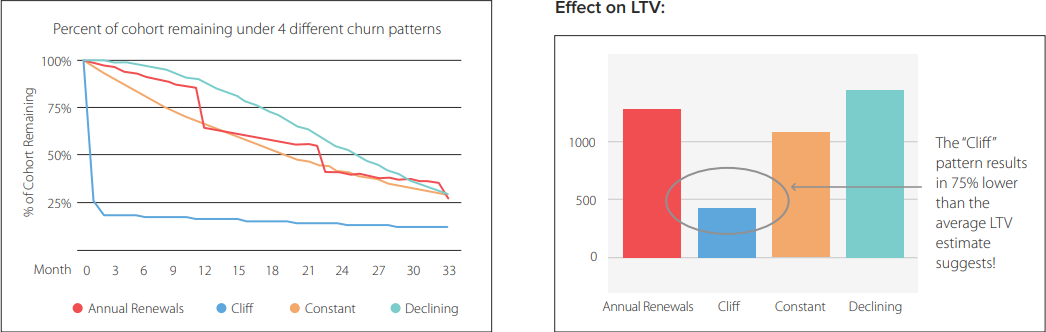
\includegraphics[scale=0.4]{churnltv}
\end{frame}

\begin{frame}\frametitle{Box Cox... }
content...
\end{frame}

\subsection{Survival Analysis}
\begin{frame}\frametitle{Types}
content...
\end{frame}

\begin{frame}\frametitle{The Kaplan-Meier curve}
content...
\end{frame}

\begin{frame}\frametitle{The log-rank test}
content...
\end{frame}

\begin{frame}\frametitle{Cox proportional hazards regression}
content...
\end{frame}

\begin{frame}\frametitle{Parametric models}
content...
\end{frame}

\begin{frame}\frametitle{Frailty models}
content...
\end{frame}

\begin{frame}\frametitle{Competing risk models}
content...
\end{frame}

\begin{frame}\frametitle{Discrete Time Model using logistic regression}
content...
\end{frame}



\subsection{Social Network Analysis}
\begin{frame}\frametitle{Social Network Analysis}
content...
\end{frame}

\subsection{Other Analysis}
\begin{frame}\frametitle{Whale Curve Analysis}
Technique to visualize the data\\
Sort the data before plotting\\
\textbf{Pareto Principle}: for many events, roughly 80\% of the effects come from 20\% of the causes\\
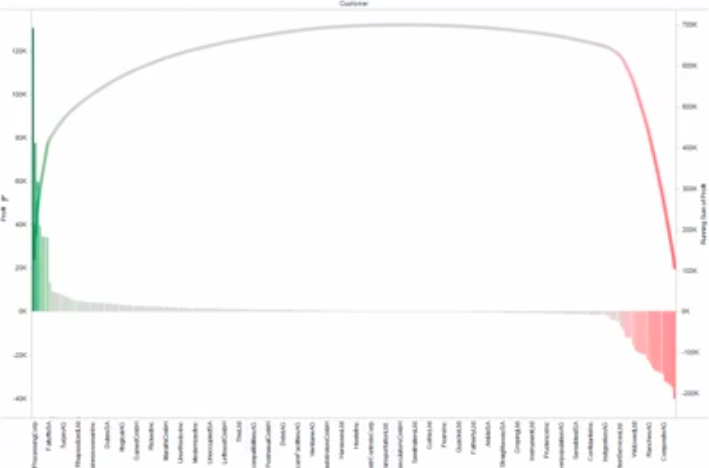
\includegraphics[scale=0.3]{other/whalecurve}

\end{frame}

\begin{frame}\frametitle{"Loss Leader” Model}

"Loss Leader” Model, where you introduce new customers at a high cost in the hope of building a customer base or securing future revenue? 

\end{frame}

\begin{frame}\frametitle{Market Basket Analysis}
content...
\end{frame}

%\subsection{}
\begin{frame}\frametitle{Propensity of Cross-sell}
content...
\end{frame}




\begin{frame}
\Huge{\centerline{Thank You!}}
\end{frame}

%----------------------------------------------------------------------------------------

\end{document} 